% Template for PLoS
% Version 3.1 February 2015
%
% To compile to pdf, run:
% latex plos.template
% bibtex plos.template
% latex plos.template
% latex plos.template
% dvipdf plos.template
%
% % % % % % % % % % % % % % % % % % % % % %
%
% -- IMPORTANT NOTE
%
% This template contains comments intended 
% to minimize problems and delays during our production 
% process. Please follow the template instructions
% whenever possible.
%
% % % % % % % % % % % % % % % % % % % % % % % 
%
% Once your paper is accepted for publication, 
% PLEASE REMOVE ALL TRACKED CHANGES in this file and leave only
% the final text of your manuscript.
%
% There are no restrictions on package use within the LaTeX files except that 
% no packages listed in the template may be deleted.
%
% Please do not include colors or graphics in the text.
%
% Please do not create a heading level below \subsection. For 3rd level headings, use \paragraph{}.
%
% % % % % % % % % % % % % % % % % % % % % % %
%
% -- FIGURES AND TABLES
%
% Please include tables/figure captions directly after the paragraph where they are first cited in the text.
%
% DO NOT INCLUDE GRAPHICS IN YOUR MANUSCRIPT
% - Figures should be uploaded separately from your manuscript file. 
% - Figures generated using LaTeX should be extracted and removed from the PDF before submission. 
% - Figures containing multiple panels/subfigures must be combined into one image file before submission.
% For figure citations, please use "Fig." instead of "Figure".
% See http://www.plosone.org/static/figureGuidelines for PLOS figure guidelines.
%
% Tables should be cell-based and may not contain:
% - tabs/spacing/line breaks within cells to alter layout or alignment
% - vertically-merged cells (no tabular environments within tabular environments, do not use \multirow)
% - colors, shading, or graphic objects
% See http://www.plosone.org/static/figureGuidelines#tables for table guidelines.
%
% For tables that exceed the width of the text column, use the adjustwidth environment as illustrated in the example table in text below.
%
% % % % % % % % % % % % % % % % % % % % % % % %
%
% -- EQUATIONS, MATH SYMBOLS, SUBSCRIPTS, AND SUPERSCRIPTS
%
% IMPORTANT
% Below are a few tips to help format your equations and other special characters according to our specifications. For more tips to help reduce the possibility of formatting errors during conversion, please see our LaTeX guidelines at http://www.plosone.org/static/latexGuidelines
%
% Please be sure to include all portions of an equation in the math environment.
%
% Do not include text that is not math in the math environment. For example, CO2 will be CO\textsubscript{2}.
%
% Please add line breaks to long display equations when possible in order to fit size of the column. 
%
% For inline equations, please do not include punctuation (commas, etc) within the math environment unless this is part of the equation.
%
% % % % % % % % % % % % % % % % % % % % % % % % 
%
% Please contact latex@plos.org with any questions.
%
% % % % % % % % % % % % % % % % % % % % % % % %

\documentclass[10pt,letterpaper]{article}
\usepackage[top=0.85in,left=2.75in,footskip=0.75in]{geometry}

% Use adjustwidth environment to exceed column width (see example table in text)
\usepackage{changepage}

% Use Unicode characters when possible
\usepackage[utf8]{inputenc}

% textcomp package and marvosym package for additional characters
\usepackage{textcomp,marvosym}

% fixltx2e package for \textsubscript
\usepackage{fixltx2e}

% amsmath and amssymb packages, useful for mathematical formulas and symbols
\usepackage{amsmath,amssymb}

% cite package, to clean up citations in the main text. Do not remove.
\usepackage{cite}

% Use nameref to cite supporting information files (see Supporting Information section for more info)
\usepackage{nameref,hyperref}

% line numbers
\usepackage[right]{lineno}

% ligatures disabled
\usepackage{microtype}
\DisableLigatures[f]{encoding = *, family = * }

% rotating package for sideways tables
\usepackage{rotating}

\usepackage{verbatim}   % useful for program listings

% Remove comment for double spacing
%\usepackage{setspace} 
%\doublespacing

% Text layout
\raggedright
\setlength{\parindent}{0.5cm}
\textwidth 5.25in 
\textheight 8.75in

% Bold the 'Figure #' in the caption and separate it from the title/caption with a period
% Captions will be left justified
\usepackage[aboveskip=1pt,labelfont=bf,labelsep=period,justification=raggedright,singlelinecheck=off]{caption}

% Use the PLoS provided BiBTeX style
% \bibliographystyle{plos2015}
\bibliographystyle{apalike}

% Remove brackets from numbering in List of References
\makeatletter
\renewcommand{\@biblabel}[1]{\quad#1.}
\makeatother

% Leave date blank
\date{}

% Header and Footer with logo
\usepackage{lastpage,fancyhdr,graphicx}
\usepackage{epstopdf}
\pagestyle{myheadings}
\pagestyle{fancy}
\fancyhf{}
\lhead{
\includegraphics[width=2.0in]{PLOS-submission.eps}}
\rfoot{\thepage/\pageref{LastPage}}
\renewcommand{\footrule}{\hrule height 2pt \vspace{2mm}}
\fancyheadoffset[L]{2.25in}
\fancyfootoffset[L]{2.25in}
\lfoot{\sf PLOS}

%% Include all macros below

\newcommand{\lorem}{{\bf LOREM}}
\newcommand{\ipsum}{{\bf IPSUM}}

%% END MACROS SECTION


\begin{document}
\vspace*{0.35in}

% Title must be 250 characters or less.
% Please capitalize all terms in the title except conjunctions, prepositions, and articles.
\begin{flushleft}
{\Large
\textbf\newline{Filament Recycling and Sustained Contractile Flows in an Actomyosin Cortex}
}
\newline
% Insert author names, affiliations and corresponding author email (do not include titles, positions, or degrees).
\\
William McFadden\textsuperscript{1},
Jonathan Michaux\textsuperscript{2},
Patrick McCall\textsuperscript{3},
Edwin Munro\textsuperscript{2,*}
\\
\bigskip
\bf{1} Biophysical Sciences Program, University of Chicago, Chicago, IL, USA
\\
\bf{2} Department of Molecular Genetics and Cell Biology, University of Chicago, Chicago, IL, USA
\\
\bf{3} Department of Physics, University of Chicago, Chicago, IL, USA
\\
\bigskip

% Insert additional author notes using the symbols described below. Insert symbol callouts after author names as necessary.
% 
% Remove or comment out the author notes below if they aren't used.
%
% Primary Equal Contribution Note
%\Yinyang These authors contributed equally to this work.

% Additional Equal Contribution Note
% Also use this double-dagger symbol for special authorship notes, such as senior authorship.
%\ddag These authors also contributed equally to this work.

% Current address notes
%\textcurrency a Insert current address of first author with an address update
% \textcurrency b Insert current address of second author with an address update
% \textcurrency c Insert current address of third author with an address update

% Deceased author note
%\dag Deceased

% Group/Consortium Author Note
%\textpilcrow Membership list can be found in the Acknowledgments section.

% Use the asterisk to denote corresponding authorship and provide email address in note below.
* emunro@uchicago.edu

\end{flushleft}
% Please keep the abstract below 300 words
\section*{Abstract}
Fill in abstract later.


% Please keep the Author Summary between 150 and 200 words
% Use first person. PLOS ONE authors please skip this step. 
% Author Summary not valid for PLOS ONE submissions.   
\section*{Author Summary}
In this paper, we develop and analyze a minimal model for 2D active networks based on the cortical cytoskeleton of eukaryotic embryos.  Our model introduces a drag-like slip between cross-linked filaments as means to dissipate stored stress, generating a macroscopic effective viscosity.  We further introduce an active friction to active stress from microscopic properties.  We generate computational simulations based on the model, and demonstrate that active stress is sufficient to drive network contraction only temporarily.  By introducing filament recycling, we are able to set up steady state flow profiles such as those found in the cortex of developing embryos and migrating cells.  The model is used to calculate phenomenological constants measured in prior experiments.  Our analysis sheds insight on potential microscopic control parameters governing broad qualitative differences in 2D active networks.  We make our model freely accessible and our methodology transparent to enable other researchers to clearly understand our modeling framework and to build upon our findings.

\linenumbers

\section*{Introduction}

\paragraph{}  Cortical flow is a fundamental and ubiquitous form of cellular deformation that underlies cell polarization, cell division, cell crawling and multicellular tissue morphogenesis\cite{cellmech_flows3,cellmech_flows2}.  These flows arise within the actomyosin cortex, a thin layer of cross-linked actin filaments and myosin motors that lies just beneath the plasma membrane \cite{Salbreux2012536}. The active forces that drive cortical flows are thought to be generated by myosin motors pulling against individual actin filaments \cite{Munro2004413}. These forces must be integrated within cross-linked networks to build macroscopic contractile stress.  At the same time, cross-linked networks resist deformation and this resistance must be dissipated by network remodeling to allow macroscopic network deformation and flow.  How force production and dissipation depend on motor activity, network architecture and remodeling remains poorly understood.

Current models for cortical flow rely on coarse-grained descriptions of actomyosin networks as active fluids, whose motions are driven by gradients of active contractile stress and opposed by an effectively viscous resistance\cite{cellmech_flows}.  In these models, gradients of active stress are assumed to reflect spatial variation in motor activity and viscous resistance is assumed to reflect the internal dissipation of elastic resistance due to local remodeling of filaments and/or cross-links \cite{PhysRevLett.106.028103}.  A key virtue of these models is that their behavior is governed by a few parameters (active stress and effective viscosity).  By coupling an active fluid description to simple kinetic models for network assembly and disassembly and making active stress and effective viscosity depend on e.g network density and turnover rates, it is possible to capture phenomenological descriptions of cortical flow.  Models based on this active fluids description can successfully reproduce spatiotemporal dynamics of cortical flow observed during polarization \cite{cellmech_flows}, cell division \cite{Turlier2014114,PhysRevLett.103.058102}, cell motility \cite{Keren:2009aa,RevModPhys.85.1143} and tissue morphogenesis \cite{Heisenberg2013948}.  

However, to understand how cells exert physiological control over cortical deformation and flow, or to build and tune networks with desired properties {\em in vitro}, it is essential to connect this coarse-grained description to the microscopic origins of force generation and dissipation within cross-linked actomyosin networks.  Both active stress and effective viscosity depend sensitively on microscopic parameters including densities of filaments, motors and cross-links, force-dependent motor/filament interactions, cross-link dynamics and network turnover rates.  Thus a key challenge is to understand how tuning these microscopic parameters controls the dynamic interplay between active force generation and passive relaxation to control macroscopic dynamics of cortical flow.

\paragraph{} Studies in living cells have documented fluid-like stress relaxation on timescales of 10-100s of seconds \cite{cellmech_flows,cellmech_flows2,cellmech_flows3,rheo_fluid,rheo_fluid2,cell_rheo_exp}.  These modes of stress relaxation are thought to arise both from the transient binding/unbinding of individual cross-links and from the turnover (assembly/disassembly) of actin filaments (ref).  Studies of cross-linked and/or bundled actin networks {\em in vitro} suggest that cross-link unbinding may be sufficient to support viscous relaxation (creep) on very long timescales\cite{rheo_cross-linksmatter,rheo_cross-linkslip1,rheo_cross-linkslip2,rheo_cross-linkslip3,rheo_nonaffine}, but is unlikely to explain the rapid large scale cortical deformation and flow observed in living cells.  suggest that rapid actin turnover must play a significant role as well. Indeed, photokinetic and single molecule imaging studies studies reveal rapid turnover of cortical actin filaments in living cells on timescales of 10-100 seconds \cite{Robin:2014aa}. Previous theoretical models have explored  the dependence of stress relaxation on cross-link binding and unbinding analytically \cite{theo_cross-linkslip1,theo_cross-linkslip2} and others have explicitly modeled reversible cross-linking in combination with complex mechanics of filament bundles \cite{model_taeyoon,rheo_cross-linkslip2,theo_cross-linkslip3}.  However, until very recently \cite{Mak:2016aa} very little attention has been paid to actin turnover as mechanism of stress relaxation. 

Recent work has also begun to reveal insights into mechanisms that govern active stress generation in disordered actomyosin networks. In vitro studies have confirmed that local interactions among actin filaments and myosin motors are sufficient to drive macroscopic contraction of disordered networks \cite{rheo_2D1}.  Theoretical studies suggest that asymmetrical compliance of actin filaments (stiffer under extension than compression) and spatial differences (dispersion) in motor activity are sufficient conditions for contraction in one \cite{1367-2630-14-3-033037} and two \cite{PhysRevX.4.041002} dimensional networks, although other routes to contractility may also exist \cite{PhysRevX.4.041002}.  Further work has explored how modulation of network architecture, cross-link dynamics and motor density, activity and assembly state can shape rates and patterns of network deformation \cite{10.1371/journal.pone.0039869,Alvarado:2013aa,C0SM00494D} or network rheology \cite{0295-5075-85-1-18007,rheo_active}.  

Significantly, {\em in vitro} models for disordered actomyosin networks have used stable actin filaments, and these networks  support only transient contraction, either because of network collapse (ref), or buildup of elastic resistance (ref?), or because network rearrangements (polarity sorting) dissipate the potential to generate contractile force (ref). This suggest that continuous turnover of actin filaments may play a key role in allowing sustained deformation and flow (refs). Recent theoretical and modeling studies have begun to explore how this could work \cite{2015arXiv150706182H,Mak:2016aa,10.1371/journal.pone.0000696}, and to explore dynamic behaviors that can emerge in contractile material with turnover \cite{PhysRevLett.113.148102}. However, there is much to learn about how the buildup and maintenance of contractile force during continuous deformation and flow depends local interplay of network architecture, motor activity and filament turnover.



\paragraph{}  The goal of this work was to build a computational bridge between the microscopic description of cross-linked actomyosin networks and the coarse grained macroscopic description of an active fluid.  We sought to capture the essential microscope features (dynamic cross-links, active motors and semi flexible actin filaments with asymmetric compliance and continuous filament recycling), but in a way that is sufficiently simple to allow systematic exploration of how parameters that govern network deformation and flow in an active fluid theory depend on microscopic parameters. To this end, we introduce several coarse-grained approximations into our representation of filament networks. First, we represent semi-flexible actin filaments as chains of simple springs with asymmetric compliance (stronger in extension than compression). Second, we replace  dynamic binding/unbinding of elastic cross-links with a coarse-grained representation in terms of molecular friction \cite{theo_friction,theo_frictionSam,theo_molefric}, such that filaments can slide past each other against a constant fictional resistance. Third, we used a similar scheme to introduce active motors at filament crossover points with a simple linear force/velocity relationship, and we introduce ?dispersion? of motor activity by making only a subset of filament overlaps active \cite{theo_frictionShila}.  Finally, we model filament turnover by regularly reseting a subset of filaments to a new unstrained position. Importantly, these simplification allows us to extend our single polymer models to dynamical systems of larger network models for direct comparison between theory and modeling results. This level of coarse graining will therefore make it easier to understand classes of behavior for varying compositions of cross-linked filament networks. In addition, it allows us to compute a new class of numerical simulations efficiently, which gives us concrete predictions for behaviors in widely different networks with measurable dependencies on molecular details. 
  

% You may title this section "Methods" or "Models". 
% "Models" is not a valid title for PLoS ONE authors. However, PLoS ONE
% authors may use "Analysis" 
\section*{Models}

\begin{figure}[h!]
\centering
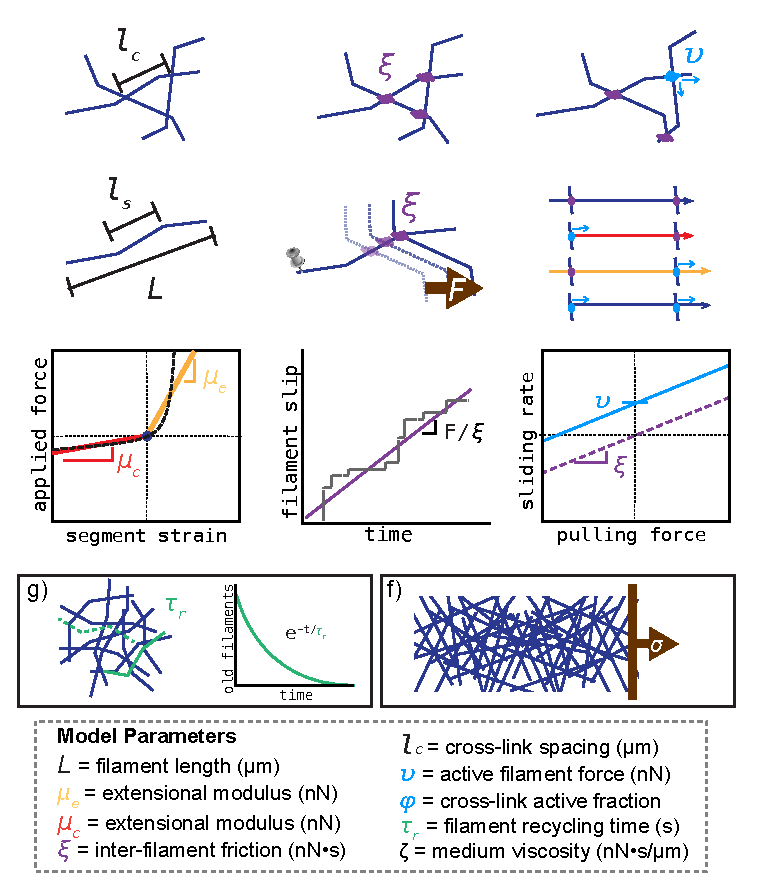
\includegraphics[width=\hsize]{figures/fig2/fig2}
\caption{\label{fig:sim} Schematic of modeling framework. a) Asymmetric filament compliance.Filaments have smaller spring constant for compression than for extension. b) Cross-link slip. Cross-links are coupled by an effective drag, such that their relative motion is
proportional to any applied force. c) Motor activity. Filament activity manifests as a basal sliding rate even in the absence of an external force. d) Fractional activity. Only a subset of filament cross-links are active, resulting in differential force exertion along the filament. e) Filament recycling. Filaments are turned over at a constant rate, leading to a refreshing in the strain state of all filaments after a characteristic timescale.}
\end{figure}

Our goal was to model essential microscope features of cross-linked actomyosin networks (semi flexible actin filaments with asymmetric compliance, dynamic cross-links, active motors and and continuous filament recycling), in a way that is simple enough to allow systematic exploration of how tuning these microscopic features controls macroscopic network deformation and flow. We focus on 2D networks for computational tractability and because they capture a reasonable approximation of the quasi-2D cortical actomyosin networks that govern flow and deformation in many eukaryotic cells\cite{cellmech_flows}, or the quasi-2D networks used in recent in vitro studies\cite{rheo_2D1,rheo_2D2}.


\subsection*{Asymmetric Filament Compliance}
We model individual filaments as chains of springs with relaxed length $l_s$.  Filaments can therefore be represented as a sequence of nodes with positions $\mathbf{x_i}$ and nearest neighbor force interactions, $\mathbf{F^{\mu}_i}$, of the form

\begin{equation}
\label{eqn:spring}
|F^{\mu}_i| = \mu\cdot\frac{|\mathbf{x_{i+1}}-\mathbf{x_i}|-l_s}{l_s} +\mu\cdot\frac{|\mathbf{x_{i-1}}-\mathbf{x_i}|-l_s}{l_s}
\end{equation}





where the modulus, $\mu$, is a composite quantity representing both filament and cross-linker compliance in a manner similar to a proposed effective medium theory \cite{theo_cross-linknonlinear}.   To model asymmetric filament compliance, we assign the modulus $\mu$, a different value depending on whether $|\mathbf{x_{i-1}}-\mathbf{x_i}|-l_s$ (the strain) is greater or less than 0. In the limit of highly rigid cross-links and flexible filaments, our model reduces to the pure semi-flexible filament models of \cite{theo_hlm,theo_hlm2}.  In the opposite regime of nearly rigid filaments and highly flexible cross links, our method is still largely similar to the model of \cite{theo_cross-linknonlinear} in small strain regimes before any nonlinear cross link stiffening.  In a departure from those models, we assume here that the magnitude of the force on interior cross-links is the same as those on the exterior.  This approach ignores the variation in strain on these two sets of cross-links as addressed in \cite{theo_cross-linknonlinear}, but we choose to ignore this variation in favor of an approximated, global mean approach.  



\subsection*{Drag-like Coupling Between Overlapping Filaments}
\label{exp_drag}
Previous models represent cross-linkers as elastic connections between pairs of points on neighboring filaments that appear and disappear with either fixed or strain-dependent probabilities (ref).  Here, we introduce a simpler coarse-grained model for dynamic cross-links by replacing many transient elastic interactions with an effective drag-like coupling between every pair of overlapping segments.
\begin{equation}
\label{eqn:drag}
\mathbf{F^{\xi}_i} = \xi \cdot \int^{s_{i+1}}_{s_{i-1}} ds \frac{l_s-|s-s_i|}{l_s} \: (\mathbf{v_i}-\mathbf{v_j}) \: p_{ij}(s)
\end{equation}

Where $p_{ij}(s)$ represents the locational distribution of cross-link points (equal to 1 at locations of cross-links and 0 elsewhere) and $\mathbf{v_i}$ and $\mathbf{v_j}$ represent the velocities of the $i$th and $j$th filament segment.  This model assumes a linear relation between applied force and the velocity difference between attached segments.  This drag-like coupling has been shown to be an adequate approximation in the case of ionic cross-linking of actin\cite{mol_fric,theo_hydroish2}, and can be found in the theoretical basis of force-velocity curves for myosin bound filaments\cite{theo_frictionShila}. Although non-linearities can arise through force dependent detachment kinetics and/or non-linear force extension of cross-links, we assume that inhomogeneities from non-linear effects are of second or higher order. With this assumption, the motion of filaments can be described by a dynamical equation of the form

\begin{equation}
\label{eqn:syst1}
L\zeta\mathbf{ v_i} +\mathbf{F^{\xi}_i}= \mathbf{F^{\mu}_i}
\end{equation}

Here, the first term in the integral is the filament's intrinsic drag through its embedding fluid, $\zeta$, while the second comes from the drag-like coupling between filaments, $\xi$.  

\subsection*{Active Coupling for Motor Driven Filament Interactions}

To add motor activity we select a subset of cross-linked points and impart an additional force of magnitude $\upsilon$ directed in the orientations of the individual filaments, $\mathbf{u_i}$.  This leads to a modification of the equation of motion to

\begin{equation}
\label{eqn:moto}
\mathbf{F^{\upsilon}_i}= \mathbf{\hat{u}_i}\cdot\upsilon\int ds \sum _j \:  \frac{l_s-|s-s_i|}{l_s} p_{ij}q_{ij}
\end{equation}

In this formulation, only at the subset of points where  $p_{ij}=1$ and $q_{ij}=1$ will there be a force imparted.  In our simulations we let $q_{ij}$ be selected randomly such that $\bar{q}=\phi$, where $\bar{q}$ indicates the mean of $q$.

Finally, for each active force, $\mathbf{F^{\upsilon}_j}$, imparted by filament $j$, we must also impart the opposite force onto the filament $i$ as well.  Therefore, the entire force balance equation with activity will appear as

\begin{equation}
\label{eqn:syst3}
L\zeta\mathbf{ v_i} +\mathbf{F^{\xi}_i}= \mathbf{F^{\mu}_i}+\mathbf{F^{\upsilon}_i} - \sum_{j}\mathbf{F^{\upsilon}_j}p_{ij}q_{ij}
\end{equation}

\subsection*{2D Network Formation}

We used a mikado model approach \cite{Unterberger2014} to initialize a minimal network of connected unstressed linear filaments in a rectangular 2D domain. We generate 2D networks of these semi-flexible filaments by laying down straight lines of length, L, with random position and orientation. We then assume that overlapping filaments become cross-linked at their point of overlap. Although real cytoskeletal networks may form with non-negligible anisotropy, we focus on isotropically initialized networks for simplicity. We define the density using the average distance between cross-links along a filament, $l_c$. A simple geometrical argument can then be used to derive the number of filaments filling a domain as a function of $L$ and $l_c$\cite{theo_hlm}.  Here, we use the approximation that the number of filaments needed to tile a rectangular domain of size $W \times H$  is $2WH/Ll_c$, and that the length density is therefore simply, $1/l_c$. In the absence of cross-link slip, we expect the network to form a connected solid with a well defined elastic modulus\cite{theo_hlm,theo_hlm2}.  


\subsection*{System of Equations for Applied Stress}
We model our full network as a coupled system of differential equations satisfying \ref{eqn:syst3}.  Although the general mechanical response of this system may be very complex, we focus our attention on low frequency deformations and the steady-state creep response of the system to an applied stress.  To do this we introduce a fixed stress, $\sigma$ along one edge of the network.  The stress is applied via individual forces to the filaments lying within a patch of size $D_w$ such that the sum of individual forces is equal to the applied stress times the height of the domain.  These forces points in the direction, $\mathbf{\hat{x}}$, producing and extension of the patch.

Finally, we add a 0 velocity constraint at the other edge of our domain of interest.  We assume that our network is in the "dry," low Reynold's number limit, where inertial effects are so small that we can equate our total force to 0.  Therefore, we have a dynamical system of wormlike chain filaments satisfying

\begin{equation}
\label{eqn:systfull}
L\zeta\mathbf{ v_i} +\mathbf{F^{\xi}_i(v_i)}= \mathbf{F^{\mu}_i(x_i)}+\mathbf{F^{\upsilon}_i(x_i)} + \sigma\mathbf{\hat{u}(x_i)}
\end{equation}

subject to constraints such that $\mathbf{v_i(x)}$ is 0 with $x=0$.  This results in an implicit differential equation for filament segments which can be discretized and integrated in time to produce a solution for the motion of the system.


\subsection*{Filament Recycling as a model for rapid filament turnover}

In living cells, actin filament assembly is governed by multiple factors that control nucleation, elongation and filament branching. Likewise filament disassembly is governed by multiple factors that promote filament severing and monomer dissociation at filament ends. Here, we focus on a lowest order model for filament recycling in which entire filaments appear with a fixed probability per unit area per unit time and disappear with a fixed probability per filament per unit time. With this assumption, in the absence of network deformation, the density of filaments will equilibrate to a steady state density with time constant $\tau_r = 1/r_{diss}$.   In deforming networks, the density will be set by a competition between strain thinning or thickening, and density equilibration via turnover. To implement this assumption, at fixed time interval $\tau_s < 0.01\cdot\tau_r$ (i.e. 1\% of the equilibration time), we selected a fraction, $\tau_s/\tau_r$, of existing filaments (i.e. less than 1\% of the total filaments) for degradation. We then generated an equal number of new unstrained filaments to appear within the network at random positions and orientations. This has the effect of creating an approximately exponential decay (with time constant $\tau_r$) in the number of old filaments over time, while maintaining a constant number of total filaments.


\subsection*{Computational Simulation Method}

Details of our simulation approach can be found in the Appendix. Briefly, equations \ref{eqn:spring},\ref{eqn:drag},\ref{eqn:moto} and \ref{eqn:systfull} define a coupled system of ordinary differential equations for the velocities of the endpoints of filament segments, $\mathbf{x}$.  These equations are coupled by the effective cross-link friction on segment overlap points, yielding a system of the form:

\begin{equation}
\mathbf{A \cdot \dot x} = \mathbf{f(x)}
\end{equation}

where $\mathbf{A }$ represents a coupling matrix between endpoints of filaments that overlap, and $\mathbf{f(x)}$ is the spring force between pairs of filament segment endpoints.   We numerically integrated this system of equations to find the time evolution of the positions of all filament endpoints. We generate a network of filaments with random positions and orientations as described above within a domain of size $D_x$ by $D_y$.  For all simulations, we imposed periodic boundaries in the y-dimension. To impose an extensional stress, we constrained all filament segment endpoints within a fixed distance $0.05\cdot D_x$ from the left edge of the domain to be non-moving, then we imposed a rightwards force on all segment endpoints within a distance $0.05\cdot D_x$ from the left edge of the patch.   To simulation free contraction, we removed all constraints at boundaries; to assess buildup of contractile stress under isometricc conditions, we pinned both left and right edges of the network as described above.




We smoothed all filament interactions, force fields, and constraints over small regions such that the equations contained no sharp discontinuities. The nominal units for length, force, and time are $\mu m$, nN, and s, respectively.  We explored parameter space around an estimate of biologically relevant parameter values given in Table \ref{table:para}. 

\begin{table}[h]
\centering
\caption{Simulation Parameter Values}
\label{table:para}
\begin{tabular}{|c|c|c|c|c|}
\hline
{\bf parameter}             & {\bf symbol} & {\bf physiological estimate}          \\ \hline
extensional modulus         & $\mu_e$        & $10 nN $                                               \\
compressional modulus             & $\mu_c$     & $ 0.1 nN $                           \\
cross-link drag coefficient & $\xi$      & $unknown $              \\
medium drag coefficient     & $\zeta$        & $0.0005 \frac{nN s}{\mu m^2} $      \\
filament length             & L            & $5 \mu m$                                          \\
cross-link spacing          & $l_c$        & $0.5 \mu m$                                         \\
domain size                 & $D_x\times D_y$            & $20\times 50 \mu m$                                 \\ \hline
\end{tabular}
\end{table}



% Results and Discussion can be combined.
\section*{Results and Discussion}
We used our model to characterize how rates and patterns of cortical flow are shaped by complex dependencies of active force generation and passive force dissipation on network architecture, local coupling (active and passive) between filaments and filament recycling.  We proceeded in three steps:  First, we analyze the passive deformation of a network in response to a constant external force.  We determine the timescales on which fluid-like deformation occurs as a function of network architecture and filament recycling times.  Next, we considered the active case and made similar measurements of the timescales of internal stress buildup and dissipation. Finally, we were able to synthesize our understanding of the passive and active systems to analyze the behavior of a more complex situation of an actively flowing network.


% PASSIVE SECTION
\subsection*{Filament recycling prevents cortical tearing and modulates the viscous stress relaxation of passive filament networks}
 
% Example of passive simulation measurements
\paragraph{Networks with passive cross-links and no filament turnover undergo three stages of deformation in response to an extensional force.} 
To characterize the passive response of a filament network with effective cross-link drag in the absence of filament recycling and motor activity, we imposed an external force on a simulated network, and then quantified network deformation and internal network stress as a function of time. An example of such simulations is shown in Figure \ref{fig:passive_ex}a.  We measured the local velocity of the network at different positions along the axis of deformation as the mean velocity of all filament segments intersecting that position;  We measured the internal network stress at each position by summing the axial component of the tensions on all filament segments intersecting that position, and dividing by network height;  finally, we measured network strain rate as the change in filament position length divided by its original position.   

We found in our measurements of instantaneous stress and velocity (Figure \ref{fig:passive_ex}b) that the network deforms nearly continuously.  During intermediate stages of the deformation, the stress profile (blue) is nearly constant throughout the material while the velocity profile (orange) is linear in space.  This justifies a material description in terms of bulk quantities, and allows us to describe the deformation field with a single approximately uniform strain rate.

Plotting the material stress and strain rates as function of time revealed that the deformation occurred in three qualitatively distinct phases (Figure \ref{fig:passive_ex}a,c). On short timescales the network exhibited a rapid viscoelastic response, characterized by a rapid buildup of internal stress and a rapid, exponential approach to a fixed strain similar to that predicted by \cite{theo_hlm}. On intermediate timescales, the internal stress remained constant while the network continued to deform slowly and continuously with nearly constant strain rate as filaments slipped past one another against the effective drag. This linear relationship between strain and time characterizes a material with an effective viscosity, $\eta_c$, given by the ratio of the applied stress to the strain rate.  We define the transition time between this fast, viscoelastic response and the slower, effectively viscous deformation phase as ($\tau_c$).  Finally, on long timescales, this effectively viscous behavior broke down.  As the network strain approached a critical value ($\sim 30\%$ for the simulation in Figure \ref{fig:passive_ex}), strain thinning lead to decreased network connectivity, local tearing, and acceleration of the network deformation (see inset in Figure \ref{fig:passive_ex}c). This eventually resulted in the highly heterogeneous network structure shown in the t=440 example of Figure \ref{fig:passive_ex}a. 


\begin{figure}[h!]
\centering
\includegraphics[width=\hsize]{figures/figure3a}
\caption{\label{fig:passive_ex}  Networks with passive cross-links and no filament turnover undergo three stages of deformation in response to an extensional force.   \textbf{a)} Three successive time points from a simulation of a $4\times10\: \mu m$ network deforming under an applied extensional stress of 0.005 $nN/\mu m$. In this and all subsequent figures, filaments are color-coded with respect state of stress (blue = tension, red = compression).  Network parameters: $L=1\: \mu m$, $l_c=0.3\: \mu m$, $\xi=100\: nN\cdot s$. \textbf{b)} Mean filament stress and velocity profiles for the  network in (a) at t=88s. Note that the stress is nearly constant and the velocity is nearly linear as predicted for a viscous fluid under extension.  \textbf{c)} Plots of the mean stress and strain
vs time for the simulation in (a), illustrating the three stages of deformation: (i) A fast initial phase accompanies rapid buildup of internal network stress; (ii) after a characteristic time $\tau_c$ s (indicated by vertical dotted line) the network deforms like a material with a constant effective viscosity, $\eta_c$, as indicated by the slope of the dashed line.  (inset) At long times, the strain accelerates as the network undergoes strain thinning and eventually tears. }
\end{figure}

% Viscosity and timescale parameter dependence
\paragraph{Network architecture sets the rate and timescales of deformation.}  To better understand the origins of effective viscosity and the timescale for transition to viscous behavior and the effective viscosity, we systematically varied network parameters and applied stress and measured effective viscosity and the transition time ($\tau_c$). For the entire range of network parameters that we sampled, we observed a transition from a fast viscoelastic response to slow effectively viscous deformation. A simple theoretical analysis predicted that the effective viscosity should be proportional to the square of the cross-link density and the effective cross-link drag coefficient of the individual cross-links, with a constant of proportionality $\pi/4$. As shown in Figure \ref{fig:passive_form}a, our simulations agree well with the theory for a large range of network parameters. For many simple viscoelastic materials, the ratio of the elastic modulus, $G_0$, to the viscosity $\eta_c$, is a general indicator of the transition timescale from elastic to viscous behavior (need a reference). Using the approximation of the equation for elastic modulus from \cite{theo_hlm}, $G_0 \approx \mu/l_c$, we predict a crossover time, $\tau_c \approx L^2\xi/l_c\mu$. By measuring the time at which the strain rate became nearly constant we obtained an estimate of this time for a wide variety of simulation parameters. As shown in Figure \ref{fig:passive_form}b, our approximation is in good agreement with the observed transition time. These data confirm that our model is consistent with previous models for the viscoelastic response of semi flexible polymer networks.


\begin{figure}[h!]
\centering
\includegraphics[width=\hsize]{figures/figure3b}
\caption{\label{fig:passive_form} Network architecture sets the rate and timescales of deformation. \textbf{a)} The effective viscosity depends on the drag coefficient and the density of the network. Data points are the normalized effective viscosity from simulations (effective viscosity measured in fluid phase divided by the cross link friction coefficient) vs the number of cross links per filament $(L/l_c - 1)$.  Dotted line indicates the relationship predicted by a simple theory, $\eta_c = \xi(L/l_c-1)^2$ \textbf{b)} The transition to viscous behavior occurs at a characteristic time, $\tau_c$, that is set by the ratio of the elastic modulus predicted in \cite{theo_hlm} (i.e. $G_0 \approx \mu/l_c$) to the effective viscosity, $\eta_c$.  }
\end{figure}


% Passive Recycling
\paragraph{Filament recycling rescues network tearing and modulates effective viscosity.}  We next explored how the passive network response to an applied force changed in the presence of filament recycling. To do so we ran a series of simulations with identical filament lengths and network densities and filament slip rates, while varying the rate at which filaments were reset to a refreshed, unstressed state. Increasing  filament recycling rates produced two  striking changes in the long time response of the network.. First, increasing recycling rates could prevent strain thinning, network tearing and acceleration of network strain rates observed in the absence of recycling. As an example,  for the network shown in Figure \ref{fig:passive_rec}a, strain thinning and network tearing  lead to a rapid increase in strain rate above a critical strain of $\sim40\%$. In contrast, when filaments are made to recycle with an average lifetime of 10 s, the same network, in response to the same level of applied stress, can sustain effectively viscous deformation, at a much higher strain rate (i.e. a much lower effective viscosity), for an indefinite period of time.  Plotting effective viscosity as a function of decreasing recycling times revealed sharp decrease in effective viscosity as the recycling time approached $\tau_c$, the characteristic time for transition to viscous deformation.  

An intuitive explanation of this effect is that rapid recycling increases the network?s ability to sustain the faster deformation rate that occurs during the initial viscoelastic response to applied stress. By constantly turning over strained network elements and replacing them with unstrained filaments , the network is able to dissipate stored elastic stress to maintain itself indefinitely within the viscoelastic response regime.  


To test if this is a general relationship, we plotted the normalized effective viscosity (ratio of effective viscosity with recycling to effective viscosity without recycling, $\eta_c$) vs a normalized recycling rate (recycling time scaled by $\tau_c$) for a large range of different network parameters and filament recycling times (Figure \ref{fig:rec_form}). Indeed, for a large range of network parameters, the normalized effective viscosity begins to decrease when the recycling time falls below $\tau_c$ and below this value the effective viscosity falls off linearly with recycling time.


\begin{figure}[h!]
\centering
\includegraphics[width=\hsize]{figures/figure5a}
\caption{\label{fig:passive_rec}  Filament recycling rescues network tearing and modulates effective viscosity.  \textbf{a)} Examples of $20 \times 12 \mu m$ network under 0.001 $nN/\mu m$ extensional stress with recycling ($\tau_r=10 s$) and without, ($\tau_r=\infty$).  Both images are taken when the patches had reached a net strain of 0.4.  The network with recycling doesn't appear to change shape because its components have been recycled to remain in the original domain.  Network parameters: $L=3\: \mu m$, $l_c=0.5\: \mu m$, $\xi=10\: nN\cdot s$.  \textbf{b)}  Strain buildup for networks with parameters as in a) in the presence of different filament recycling rates. Dotted line indicates the strain state at which the snapshots in panel a) were taken.  Note that the strain rate for $\tau_r=1000$ is essentially identical to that of $\tau_r=\infty$, indicating that recycling does not govern the relaxation rate if the recycling time is above a threshold.}
\end{figure}

%Discuss
Taken together, our results for the passive network under extension suggest that the passive stress relaxation of our network model is modified strongly by the presence of filament recycling. Given high enough levels of recycling, we find that network tearing can be prevented and that a steady state effective viscosity is established. Our model also suggests a simple microscopic derivation of viscosity which depends on the strength of inter filament cross-linking, the networks architecture, and the timescale of filament recycling.








% ACTIVE SECTION
\subsection*{Filament recycling allows persistent stress buildup in active networks}

\paragraph{In the absence of filament recycling, active networks with free boundaries contract and then stall against passive resistance to network compression.}


We found that our simulation axioms were able to produce transient contraction of a patch of free-floating network.  As shown in Figure \ref{fig:active_con}a, when an initially unstrained network has internal motor activity "switched on" at $t=0$, the area of the patch begins to decrease.  By 100 s, the network has contracted by 40\%, and many internal filaments can be seen to have reached a compressed state (indicated by orange).  By 150 s, the compression has stalled, but filament sliding has begun to force some filaments away from the center. Over long time periods, this filament sorting actually rearranges the entire network, undoing the initial contraction (see supplemental video).

By monitoring both the network and individual filament strains, as in Figure \ref{fig:active_con}b, we see that the networks macroscopic deformation can be explained entirely by a buildup of inward compression on individual filaments.  Due to the strong stiffness asymmetry, there is far more compressive strain than there is extension in the network. It is this asymmetry that generates the net contraction in a disordered network despite myosin activity being equally capable of generating both.  The network contraction stalled over the same timescale as individual filaments, further indicating the essential role of filament compression in generating contractility.  

The final contraction extent was strongly dependent on the magnitudes of both the filament stiffness asymmetry (i.e. the ratio of the extensional and compressive stiffnesses $\mu_e/\mu_c$) and the motor activity strength ($\upsilon$).  As shown in Figure \ref{fig:active_con}c, small stiffness asymmetries lead to less overall contraction, while larger asymmetries appear to approach some asymptotic limit once they reach a ratio of $\sim 100$.  Additionally, contraction would only occur when there was fractional motor activity, $0<\phi<1$, (see supplement).  Finally, we found that the contraction consistently stalled over a time scale, $\tau_m=$ (see supplement), indicating that the network architecture also plays a role in setting the timescale of contraction.  These findings of the minimal requirements for contractility are all in direct accordance with the theoretical predictions of \cite{1367-2630-14-3-033037} and \cite{PhysRevX.4.041002}.  In fact, we find that removing any single factor from this simulation framework leads to a loss of contraction, suggesting that this system may represent a minimal model of contractility. 

\begin{figure}[h!]
	\centering
	\includegraphics[width=\hsize]{figures/figure4a}
	\caption{\label{fig:active_con} In the absence of filament recycling, active networks with free boundaries contract and then stall against passive resistance to network compression. \textbf{a)}  Example of an active network contracting. Note the buildup of compressive stress as contraction approaches stall between 100 s and 150 s.  Network parameters: $L=5\: \mu m$, $l_c=0.3\: \mu m$, $\xi=100\: nN\cdot s$, $\upsilon=0.1\: nN$.  \textbf{b)} Plots showing time evolution of total network strain and  the average extensional (blue) or compressive (red) strain on individual filaments.   \textbf{c)} The network's ability to deform requires asymmetric filament compliance.  Total network strain also increases with the applied myosin force $\upsilon$.}
\end{figure}

\paragraph{Active networks can only exert a transient force against a fixed boundary in the absence of filament recycling.}

Due to the complication of making measurements in the presence of such large-scale rearrangements of the network, we decided to additionally analyzed the stress buildup in a patch that was constrained to maintain its original area.  The results from Figure \ref{fig:active_str}a echo those from Figure \ref{fig:active_con}a, with a consistent buildup of internal filament strain (represented by the colored lines) that stabilizes and persists indefinitely.  In contrast, the network in Figure \ref{fig:active_str}a doesn't demonstrate any apparent large-scale rearrangement as any net deformation is impossible since the patch sets in a domain with periodic boundaries.

Under these conditions, we found that a net stress was generated throughout the material, but similar to the results for contraction in Figure \ref{fig:active_con}, the net stress could not be maintained.  As shown in Figure \ref{fig:active_str}b, the net stress (black line) initially increases to a maximum $\sigma_a$, but then decays back to 0 over longer times. However, the internal compressive and extensional stresses do not decay away entirely.  Instead, after the peak stress is reached, the internal stresses become balanced leading to an apparent net stress of approximately 0 despite a nonzero internal stress.  

Finally, we measured the time of peak stress and found it consistently occurred with a characteristic time, $\tau_a=\xi/l_c\sqrt{\mu\upsilon}$, as shown in Figure \ref{fig:active_str}c. 

\begin{figure}[h!]
	\centering
	\includegraphics[width=\hsize]{figures/figure4b}
	\caption{\label{fig:active_str} In the absence of filament recycling, active networks can only exert a transient force against a fixed boundary.  \textbf{a)} Simulation of an active network with fixed boundaries illustrating progressive buildup of internal stress through local filament rearrangement and deformation. Note the progressive buildup of compressive stress on individual filaments. Network parameters: $L=5\: \mu m$, $l_c=0.3\: \mu m$, $\xi=100\: nN\cdot s$, $\upsilon=0.1\: nN$.  \textbf{b)} Plots of total network stress and the average extensional (blue) and compressive (red) stress on individual filaments for the simulation shown in (a). Rapid buildup of extensional stress allows the network transiently to exert force on its boundary, but this force is dissipated at longer times as   as internal extensional and compressive stresses become balanced. \textbf{c}. Measurement and prediction of the characteristic time ($\tau_a$) at which the maximum stress is achieved. }
\end{figure}

\paragraph{Filament recycling allows network to exert sustained stress on a fixed boundary.}
We next added filament recycling to the simulation setup with and found that the presence of recycling allowed for persistent.  Similar to the mechanism for preserving integrity in passive networks, the recycling appears to refresh the network such that subsets of filaments are continually transitioning from an unstressed to their stressed state before being recycled back to the unstressed state.  The presence of recycling therefore both repaired structural inhomogeneities and reset the net strain of individual filaments. The panels in \ref{fig:active_rec}a show the differences in structure for identical starting architectures in the presence of different recycling timescales.  Clearly, longer recycling times allow the network to reach a more strongly reorganized and internally stressed network.

Upon the addition of filament recycling, we found that the network maintained a nonzero net stress for timescales much longer than $\tau_a$.  We refer to this as the steady state stress because, based on our simulations, it doesn't appear that this stress ever subsides.   As can be seen in Figure \ref{fig:active_rec}b, The profile of stress buildup changes dramatically by changing the recycling timescale in identical networks corresponding to those in Figure \ref{fig:active_rec}a.  It's important to notice that the effect of changing recycling time is not entirely straightforward.  As the recycling time is decreased from 333 to 33.3, we can see that the long-term steady state increases from nearly 0.05 to a closer to 0.15.  Nevertheless, the final steady state is still lower than the peak stress for those curves.  In contrast, for the faster recycling rates (3.33, 0.33, 0.033), the final steady state decreases monotonically with decreasing recycling time.  In addition, for these shorter timescales, the stress never reaches a peak but rather rises immediately to its steady state level.  We attribute this to the strain resetting whereby individual filaments repeatedly are set to an unstrained state and then transition to having more strain until they are again reset.


\begin{figure}[h!]
	\centering
	\includegraphics[width=\hsize]{figures/figure5b}
	\caption{\label{fig:active_rec}  Filament recycling allows network to exert sustained stress on a fixed boundary. \textbf{a)}  Example simulations of active networks and fixed boundaries for different timescales of filament recycling. Network parameters are the same as in Figure 6, except that the active force (v = 1) has been increased to emphasize the effects of internal network remodeling under stress. Note that significant remodeling occurs for longer recycling times.  \textbf{b)} Plots of net stress for different recycling times; for long-lived filaments, stress is built rapidly, but then dissipates.  Increasing filament turnover rates reduces stress dissipation by recycling compressed filaments; however, very short recycling times prevent any stress from being built up in the first place. }
\end{figure}










% COMBINED SECTION
\subsection*{Filament recycling tunes the balance between active stress buildup and viscous stress relaxation to generate flows}
We have shown that filament recycling has a strong impact on both passive and active properties of networks.  We ultimately wish to show how filament recycling impacts flows.  Active fluid theories propose that flow can be explained in terms of the interplay between active stress and effective viscosity. Therefore, we next tested whether we could measure the effect of recycling on flow in networks with both an active and a passive domain.
 

\paragraph{Filament recycling tunes the magnitudes of both effective viscosity and steady state stress.}  
To begin, we repeated the single domain (passive or active) simulations while varying all of our networks microscopic parameters.   By exploring the effect of these parameters on the output variables we were able to determine the general form of the dependence. In Figure \ref{fig:rec_form}, we illustrate the data collapse of all our simulation results (See Supp. for details of parameter exploration).  Interestingly, both the viscosity (in Figure \ref{fig:rec_form}a) and stress (in Figure \ref{fig:rec_form}b) show changes in behaviors on either side of their respective governing timescales ($\tau_c$ for viscosity and $\tau_a$ for active stress).  Effective viscosity was found to be independent of recycling time until recycling time became of the same order as the elastic to viscous crossover timescale, at which point it decreased with decreasing recycling time.  Similarly, the steady state stress increases with increasing recycling time until it reaches the point of peak stress buildup.  From that point it decreases with increasing recycling time.


\begin{figure}[h!]
\centering
\includegraphics[width=\hsize]{figures/figure5S}
\caption{\label{fig:rec_form}  Filament recycling tunes the magnitude of effective viscosity and steady state stress. \textbf{a)}  Normalized effective viscosities as a function of the normalized recycling time. When the recycling timescale is significantly less than the passive relaxation timescale (see Figure \ref{fig:passive_form}), the viscosity of the network becomes dependent on recycling time.  \textbf{b)} Normalized steady state stress as a function of normalized recycling time.  The steady state stress is set by the timescale at which the network strain is refreshed relative to the timescale at which the max stress is reached. }
\end{figure}


\paragraph{Filament recycling allows sustained flows in networks with non-isotropic activity.}
To clearly interrogate the mutual dependencies of effective viscosity and active stress, we next combined passive and active elements in the same simulations.  As illustrated in Figure \ref{fig:flow_ex}a, we generated networks where the left side of the domain contained only passive cross-linkers, while the right side contained a mix of active and passive cross-links.  In these, network we observed a sharp dependence on filament recycling rate.  In the $\tau_r=1000$ s case, filaments deformed more extensively (orange lines), and the network developed noticeable spatial heterogeneity.  On the other hand for shorter recycling time of $\tau_r=33$ s, the network remained much more connected and filaments underwent less total compressional strain.  We measured the flow profile across the entire simulation and observed that in both cases the flow field converged on the region at the (See Supp.) in a manner highly similar to physiological flow profiles found in e.g. \textit{C. elegant} embryos.  However, there were large differences in the magnitude and duration of the resulting flows which depended on the recycling time.

To understand the time progression of the flow profile, we measured the average network strain over time.  From this measurement, we could see a sharp dependence of the behavior on the recycling time, as shown in Figure \ref{fig:rec_form}b.  For very long recycling times ($\tau_r=1000$, dark blue line), the network showed a rapid initial deformation that quickly reached its limit and stalled.  However, with decreasing filament recycling times, we found the network was able to sustain its deformation and that the long term strain rate rose toward an asymptotic limit.  At the shortest recycling timescales measured, we still saw the effective viscosity remaining relatively high, indicating that for sufficiently short recycling times the effective viscosity may approach an asymptotic flow rate.

\begin{figure}[h!]
\centering
\includegraphics[width=\hsize]{figures/figure6a}
\caption{\label{fig:flow_ex}  Filament recycling allows sustained flows in networks with non-isotropic activity. \textbf{a)} Example simulations of non-isotropic networks with long ($\tau_r=1000$) and short ($\tau_r=33$) recycling timescales. In these networks the left half of the network is passive while the right half is active.  Network parameters: $L=5\: \mu m$, $l_c=0.3\: \mu m$, $\xi=100\: nN\cdot s$, $\upsilon=1\: nN$. \textbf{b)} Graph of strain for identical networks varying recycling timescales.  With long recycling times, the network stalls; reducing the recycling timescale allows the network to persist in its deformation.  However, for the shortest recycling timescales, the steady state strain appears to approach an asymptotic limit. }
\end{figure}

\paragraph{Filament recycling enables macroscopic flows and introduces filament length control over flow rate.}
We repeated the above analysis for many more network simulation conditions. As shown in Figure \ref{fig:flow_form}a, as the recycling timescale approaches the timescale of maximum stress buildup ($\tau_a$), all networks approach a steady state strain rate.  This further supports the hypothesis that once one attains sufficiently rapid recycling, the network may remain buffered to achieving a constant flow rate.

As a final point, we wished to mention what happens when filament recycling is held constant and other parameters are changed.  Interestingly, we found surprising architectural dependence for network architectures very closely poised to our physiological estimates.  In that regime, filament length was able to tune networks between a low flow and a high flow mode with close to $1/L$ dependence.  We believe this may be due to the difference in $L$ dependence between the timescales of effective viscosity and stress buildup. 
\begin{figure}[h!]
\centering
\includegraphics[width=\hsize]{figures/figure6b}
\caption{\label{fig:flow_form}  Filament recycling enables macroscopic flows and introduces filament length control over flow rate. \textbf{a)}  Graph of network long-term strain rate as a function of recycling timescale across a wide range of parameter space.  Note that networks only begin to maintain long-term flows when the recycling time is less than $100\tau_a$. \textbf{b)} For a fixed filament recoiling time, filament length tuned network deformation rate.}
\end{figure}








%Conclusion
\section*{Conclusion}
Our work aimed to create a simulation framework that would allow us to analyze the origins of macroscopic flow in terms of a handful of physiologically relevant microscopic parameters.  Toward this aim we developed a minimalist model of a 2D filament network and analyzed the network's reaction to a variety of situations.  We found mathematical relationships that determined both the passive effective viscosity and the active stress generation of networks with and without recycling.  From these relationships we were able to make predictions about the .  

Importantly, our work brings a theoretical understanding to the importance of actomysoin turnover in producing and maintaining long-term large scale flows.  This is not entirely surprising due to the abundance of physiological mechanisms for generating network turnover.  We propose the concept of "filament recycling" to refer to the multitude of biochemical interactions which can give rise to the piece by piece architectural resetting of filament networks.  We believe that our analysis of networks in the presence of this filament recycling will be useful in further developing the qualitative and quantitative understanding the deformation of these complex networks.

\section*{Supporting Information}

% Include only the SI item label in the subsection heading. Use the \nameref{label} command to cite SI items in the text.

\section*{Acknowledgments}
We would like to thank Shiladitya Banerjee and Patrick McCall for stimulating discussions.

\nolinenumbers

%\section*{References}
% Either type in your references using
% \begin{thebibliography}{}
% \bibitem{}
% Text
% \end{thebibliography}
%
% OR
%
% Compile your BiBTeX database using our plos2015.bst
% style file and paste the contents of your .bbl file
% here.
% 
\bibliographystyle{plos2015}
\bibliography{slippage,active}

\begin{comment}
\begin{thebibliography}{10}
\bibitem{bib1}
Devaraju P, Gulati R, Antony PT, Mithun CB, Negi VS. Susceptibility to SLE in South Indian Tamils may be influenced by genetic selection pressure on TLR2 and TLR9 genes. Mol Immunol. 2014 Nov 22. pii: S0161-5890(14)00313-7. doi: 10.1016/j.molimm.2014.11.005

\bibitem{bib2}
Huynen MMTE, Martens P, Hilderlink HBM. The health impacts of globalisation: a conceptual framework. Global Health. 2005;1: 14. Available: http://www.globalizationandhealth.com/content/1/1/14.

\end{thebibliography}
\end{comment}


\end{document}

